\subsubsection{ESTAG-C}

\textbf{ESTAG-C (ESTÁGIO-DE-CRESCIMENTO-DA-PLANTA):} Em geral, a planta tem um aumento progressivo de consumo hídrico até o período de floração e frutificação. A variável  \textbf{ESTAG-C}, assume diferentes valores de acordo com o tipo de cultura e a fase de crescimento da planta.

\begin{figure}[h!]
\centering
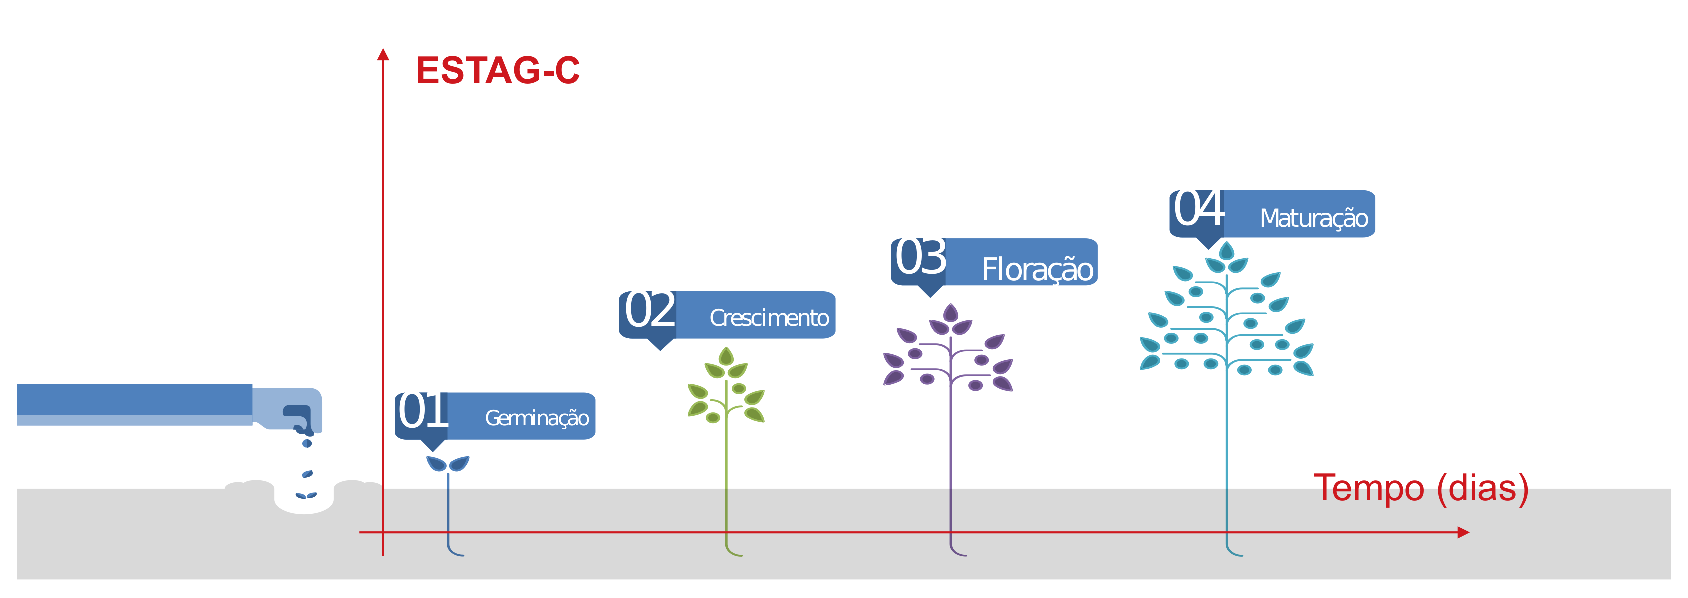
\includegraphics[width=1\linewidth]{Descricao/Imagens/estagio_de_crescimento}
\caption{}
\label{fig:estagio_de_crescimento}
\end{figure}



\begin{table}[h!]
	
	
	
	\centering
	\rowcolors{3}{lightgray}{}
	\caption{Valores médios do coeficiente de cultivo}
	\label{tab:ESTAG-C}
	\begin{tabular}{lcccc}
		\hline \hline
		\multirow{2}{*}{\textbf{Cultura}} & \textbf{Plantio-Germinação} & \textbf{Crescimento} & \textbf{Floração}  & \textbf{Maturação} \\
		& \textbf{Período 1}          & \textbf{Período 2}   & \textbf{Período 3} & \textbf{Período 4} \\
		\hline 
		Alface                   & 0,45               & 0,6         & 1         & 0,9       \\
		Cana-de-açúcar           & 0,5                & 1           & 1,1       & 0,65      \\
		Cítricos (ex. laranja)   & 0,65               & 0,7         & 1,7       & 0,65      \\
		Melão                    & 0,45               & 0,75        & 1         & 0,75      \\
		Milho                    & 0,4                & 0,8         & 1,15      & 1         \\
		Tomate                   & 0,45               & 0,75        & 1,15      & 0,8      \\
		\hline
	\end{tabular}
\end{table}


\begin{figure}[h!]
\centering
\includegraphics[width=1\linewidth]{Descricao/Imagens/ESTAG-C}
\caption{Estágio de crescimento da planta}
\label{fig:ESTAG-C}
\end{figure}

